\documentclass{article}
\usepackage{PRIMEarxiv}
\usepackage[utf8]{inputenc}
\usepackage{algorithm}
\usepackage{algpseudocode}
\usepackage{dsfont}
\usepackage[T1]{fontenc}
\usepackage{hyperref}
\usepackage{url}
\usepackage{mathtools}
\usepackage{booktabs}
\usepackage{amsfonts}
\usepackage{amsmath}
\usepackage{amssymb}
\usepackage{nicefrac}
\usepackage{microtype}
\usepackage{lipsum}
\usepackage{fancyhdr}
\usepackage{graphicx}
\graphicspath{{media/}}
\usepackage{natbib}
\usepackage{mhchem}
\usepackage{xcolor}
\usepackage{hyperref}
\hypersetup{
    colorlinks=true,
    linkcolor=blue,
    urlcolor=blue
}
\usepackage{listings}
\usepackage{xcolor}
\usepackage{tikz}
\usepackage{pgfplots}
\pgfplotsset{compat=1.18}

\definecolor{codegray}{gray}{0.95}

\lstset{
  backgroundcolor=\color{codegray},
  basicstyle=\ttfamily\small,
  keywordstyle=\color{blue},
  commentstyle=\color{gray},
  stringstyle=\color{teal},
  showstringspaces=false,
  breaklines=true,
  frame=single,
  language=Python
}


\pagestyle{fancy}
\thispagestyle{empty}
\rhead{ \textit{ }} 

\title{Linearization of the Feed-forward Layers\\ in Neural Networks}

\author{
  Lisa Wang \\
   \\
  Columbia University \\
  New York, New York \\
  \texttt{hw3082@columbia.edu} \\
    \And
  Victor Lin \\
   \\
  Columbia University \\
  New York, New York \\
  \texttt{vl2580@columbia.edu} \\
    \And
  Jicheol Ha \\
   \\
  Columbia University \\
  New York, New York\\
  \texttt{jh4762@columbia.edu}
}

\usepackage{sectsty}
\sectionfont{\fontsize{16}{16}\selectfont} % Section: font, line spacing
\subsectionfont{\fontsize{14}{14}\selectfont} % Subsection: 12pt font, 14pt line spacing
\subsubsectionfont{\fontsize{12}{12}\selectfont}

\begin{document}
\maketitle
\vspace{-0.5cm}
\begin{abstract}
In this work, we propose a functional decomposition of the Gaussian Error Linear Unit ($\operatorname{GELU}$) into two independent mappings, $\Phi(\cdot)$ and $\Psi(\cdot)$. We assume multi-dimensional inputs, specifically linear transformations of the form $Wx$, where $W$ is a square matrix and $x$ is a column vector. In the biased approach, we use the Taylor series expansion of the standard normal cumulative distribution function to  express the $\operatorname{GELU}$ as an infinite sum of scaled powers of $Wx$. Then, by using the Kronecker product, we decompose powers of $Wx$ into linear combinations of the elements of $W$ and $x$, making explicit the complex nonlinearity that $\operatorname{GELU}$ introduces. In the unbiased approach, we train $\Phi(\cdot)$ and $\Psi(\cdot)$ using a Multilayered Perceptron, which effectively addresses nonlinearities in $\operatorname{GELU}$, albeit less explicitly. The biased approach favors mathematical understanding, while the unbiased approach is machine-driven. We show that both can approximate the $\operatorname{GELU}$ well. As state-of-the-art transformer-based models use $\operatorname{GELU}$, benefits of a decomposed activation function include faster model convergence.
\end{abstract}

\keywords{Gaussian Error Linear Unit \and Kronecker Product \and Functional Decomposition \and Neural Networks \and Activation Function \and Matrix Algebra \and Taylor Series Approximation \and Multilayered Perceptron}

\section{Introduction}
The Gaussian Error Linear Unit ($\operatorname{GELU}$) is a neural network activation function that is used in several deep learning architectures. First introduced by Hendrycks and Gimpel in 2016, $\operatorname{GELU}$ is the product of an input $x$ and the probability that $x$ is greater than zero under a standard normal distribution. Mathematically, $\operatorname{GELU}(x) = x\cdot \Phi(x)$, where $\Phi$ is the standard normal cumulative distribution function. Unlike traditional activation functions such as the Rectified Linear Unit ($\operatorname{RELU}$) or the hyperbolic tangent function, $\operatorname{GELU}$ is smoother around zero, non-monotonic, and continuously differentiable for all inputs, which effectively addresses the vanishing gradient problem observed in ReLU. These properties make it particularly suitable for self-attention mechanisms and transformer architectures, where it has demonstrated superior performance compared to its predecessors. Moreover, its probabilistic nature introduces dilution and dropout that varies with the magnitude of the input signal. This characteristic becomes significant in deep transformer networks, where the interaction between self-attention mechanisms and non-linear activation functions plays a crucial role in model performance. Notable implementations include natural language processing models such as GPT (Brown et al., 2020) and BERT (Devlin et al., 2019), and computer vision models such as Vision transformers (Alexey Dosovitskiy et al., 2010). 

\section{Problem Statement}

We formally define $\operatorname{GELU}$ as the product between $x$ and the standard normal cumulative distribution function:

\begin{equation}
    \operatorname{GELU}(x) = x \int_{-\infty}^{x} \frac{t}{\sqrt{2\pi}} e^{-\frac{t^2}{2}} \; dt
    \label{eq:gelu}
\end{equation}

We want to find $\Phi: \mathbb{R}^{d \times d} \rightarrow \mathbb{R}^{d \times m}$ and $
\Psi: \mathbb{R}^d \rightarrow \mathbb{R}^m$ such that

$$
\operatorname{GELU}((Wx)_{i}) \approx \Phi(W_i)\Psi(x_i)
$$

where $(Wx)_i$ is the $i^{th}$ \textbf{element} of $Wx$, $W_i$ the $i^{th}$ \textbf{row} of $W$, and $x_i$ the $i^{th}$ \textbf{element} of $x$ for $i \in \{1,...,d\}$. We assume an element-wise operation of $\operatorname{GELU}$. 

\section{Biased Estimation}

\subsection{Mathematical basis for functional decomposition}


\subsubsection{Taylor series expansion of the standard normal cumulative distribution function}

We first express the standard normal cumulative distribution function as a Taylor series. Recall that 
$$
e^{x} = \sum_{n=0}^{\infty} \frac{x^n}{n!}
$$
Using this, 
$$
e^{-\frac{x^2}{2}} = \sum_{n=0}^{\infty} \frac{\left(-\frac{x^2}{2}\right)^n}{n!} = \sum_{n=0}^{\infty}\frac{(-1)^n x^{2n}}{2^n n!}
$$

Let $G(x)$ be the indefinite integral of the standard normal cumulative distribution function. Then, 

\begin{align*}
G(x) &\coloneqq \frac{1}{\sqrt{2\pi}}\int \sum_{n=0}^{\infty} \frac{(-1)^n x^{2n}}{2^n n!} x \; dx\\
&= \frac{1}{\sqrt{2\pi}} \sum_{n=0}^{\infty} \int \frac{(-1)^n x^{2n}}{2^n n!} x \; dx\\
&= \frac{1}{\sqrt{2\pi}} \sum_{n=0}^{\infty} \frac{(-1)^n}{2^n n!} \int x^{2n+1} \; dx\\
&= \frac{1}{\sqrt{2\pi}} \sum_{n=0}^{\infty} \frac{(-1)^n x^{2n+2}}{2^n n! (2n+2)}
\end{align*}

Now, let $F(x)$ be the standard normal cumulative distribution function. 

$$
F(x) = \int_{-\infty}^{x} \frac{1}{\sqrt{2\pi}} e^{\frac{-t^2}{2}} dt
$$

Since $F(0) = 0.5$, we see that

$$
F(x) = 0.5 + \frac{1}{\sqrt{2\pi}} \sum_{n=0}^{\infty} \frac{(-1)^n x^{2n+1}}{2^n n! (2n+1)}
$$

\subsubsection{Taylor series expansion of the Gaussian Error Linear Unit}

Using the expression from \eqref{eq:gelu}, for $x\in \mathbb{R}$,

\begin{align*}
\operatorname{GELU}(x) &= x F(x)\\
&= x \left(0.5 + \frac{1}{\sqrt{2\pi}}\sum_{n=0}^{\infty}\frac{(-1)^n x^{2n+1}}{2^n n!(2n+1)}\right)\\
&= 0.5x + \frac{1}{\sqrt{2\pi}} \sum_{n=0}^\infty \frac{(-1)^n x^{2n+2}}{2^n n!(2n+1)}
\end{align*}

Therefore, for each element in $Wx$, we have

\begin{equation}
\operatorname{GELU}((Wx)_i) = 0.5 (Wx)_i + \frac{1}{\sqrt{2\pi}}\sum_{n=0}^{\infty}\frac{(-1)^n ((Wx)_i)^{2n+2}}{2^n n!(2n+1)}
\label{eq:expanded gelu}
\end{equation}

\subsubsection{Multinomial expansion of $(Wx)_i$s}

We use the multinomial theorem to decompose the $((Wx)_i)^{2n+2}$ term in \eqref{eq:expanded gelu}, 

\begin{align*}
(Wx_i)^{2n+2} &= \left( W_i\cdot x \right)^{2n+2}\\
&= \sum_{j=1}^d W_j \cdot x_i \text{ for } j \in \{1,2,...,d\}\\
&= \sum_{\substack{k_1 + \cdots + k_r = 2n+2\\
k_1, k_2 , \ldots, k_m \geq 0
}}
    \binom{2n+2}{k_1, \ldots, k_r}
    \prod_{m=1}^r (W_{j})^{k_m}
    \prod_{m=1}^r (x_i)^{k_m}
\end{align*}

where $W_i$ is the $i^{th}$ row of $W$ and $W_j$ is the $j^{th}$ element of that row, and

$$
\binom{2n+2}{k_1, \ldots, k_r} = 
\frac{(2n+2)!}{k_1! \, k_2! \, \cdots \, k_r!}
$$

is the multinomial coefficient. Plugging this expression back to \eqref{eq:expanded gelu} completes the function decomposition, whose closed form will be expressed in a Kronecker product in \ref{subsec:general forms}.

\subsection{Biased estimation using Kronecker products}

\subsubsection{General form of approximating GELU using Taylor series}

We rewrite the Taylor series approximation of $\operatorname{GELU}(Wx)$ in a general form amenable to decomposition into $\Phi$ and $\Psi$.

Let $x_1'$ be the first component of $Wx$. Since the GELU is an element-wise operation, without loss of generality, any decomposition we find for $x_1'$ can be generalized to all dimensions.

\[
x_1' = (Wx)_1= W_1 \cdot x
\]
where $W_1$ is the first row of the weight matrix $W$ and $x$ is the input vector. 

Plugging $x_1'$ into \eqref{eq:expanded gelu}, the fully expanded GELU approximation using a finite Taylor sum is
\[
\text{GELU}(x_1') \approx \frac{x_1'}{2} + \frac{(x_1')^2}{\sqrt{2\pi}} - \frac{(x_1')^4}{6\sqrt{2\pi}} + \frac{(x_1')^6}{40\sqrt{2\pi}} - \frac{(x_1')^8}{336\sqrt{2\pi}} + \cdots
\]

which has a general form that prepares us for decomposition into $\Phi$ and $\Psi$
\begin{equation}
    a_0 (W_1 x) + a_1 (W_1 x)^2 + a_2 (W_1 x)^4 + \cdots
    \label{eq:taylor approximation general form}
\end{equation}

where $a_n$'s are the coefficients of \eqref{eq:expanded gelu}.

\subsubsection{Constructing $\Phi$ and $\Psi$ using Kronecker products}\label{subsec:general forms}

We show that each non-linear term $(W_1 x)^{2n}$ for $n=1,2,...$ can be decomposed into a dot product between the lifted versions of $W$ and $x$.

For simplicity, let $x$ be a column vector of dimension $d=2$. Then, by the multinomial theorem, the first nonlinear term of \eqref{eq:taylor approximation general form} expands to:

\begin{align}
a_1 (W_1 x)^2 
&= \left( w_1^2 x_1^2 + w_1 w_2 x_1 x_2 + w_2 w_1 x_2 x_1 + w_2^2 x_2^2 \right) \notag \\
&= a_1 \begin{pmatrix}
w_1^2 & w_1 w_2 & w_2 w_1 & w_2^2
\end{pmatrix}
\begin{pmatrix}
x_1^2 \\
x_1 x_2 \\
x_2 x_1 \\
x_2^2
\end{pmatrix}
\label{eq:multinomial expansion linear combination}
\end{align}

We can equivalently represent \eqref{eq:multinomial expansion linear combination} as a Kronecker product, a matrix operation that takes two matrices and produces a larger block matrix by multiplying each element of the first matrix by the entire second matrix.

\begin{equation*}
    a_1 \cdot (W \otimes W) \cdot (x \otimes x)^\intercal
\end{equation*}

where $\otimes$ is the Kronecker product operator.

For higher-order nonlinear terms ($n\geq2$) in \eqref{eq:taylor approximation general form}, the general Kronecker form is:
\[
a_n (W_1 x)^{2n} = a_n \cdot (W^{\otimes 2n}) \cdot (x^{\otimes 2n})^\intercal
\]

Thus, for an expanded Taylor series approximation, the decomposed functional estimation for a single output dimension corresponding to \( \text{GELU}(W_1 x) \) is given by

\[
a_0 (W_1 x) + 
a_n \left( \sum_{i=1}^d w_i x_i \right)^{2n} = a_0 (W_1 x) + a_n \cdot \left( W^{\otimes 2n} \right) \cdot \left( x^{\otimes 2n} \right)^\intercal \text{ for } n\geq 1
\]

where $w_i$ is the $i^{th}$ element of $W$.

Therefore, we propose a functional decomposition of the GELU given by
\begin{equation}
\text{GELU}(W_1 x) \approx \Phi(W) \cdot \Psi(x)^\intercal
\label{eq:kronecker_approx}
\end{equation}
where
\begin{align*}
\Phi(W) &= \sum_{n=0}^N \Phi_n(W), \quad \text{with} \quad \Phi_0(W) = a_0 \cdot W,\ \Phi_n(W) = a_n \cdot W^{\otimes 2n}\ \text{for } n \geq 1, \\
\Psi(x) &= \sum_{n=0}^N \Psi_n(x), \quad \text{with} \quad \Psi_0(x) = x,\ \Psi_n(x) = x^{\otimes 2n}\ \text{for } n \geq 1.
\end{align*}


$a_n$s are the coefficients in \eqref{eq:expanded gelu},
and $N$ is the number of terms in the finite Taylor series.
\subsubsection{Code}

\href{https://colab.research.google.com/github/v-y-l/Machine-Learning-Notebooks/blob/main/Victor's_biased_estimation_using_kronecker_products.ipynb}{
Link to Colab Notebook: Kronecker Estimator with Validation}

Using \eqref{eq:kronecker_approx}, the code performs the computation for each dimension.

\begin{lstlisting}
class TaylorSeriesGeluEstimator:
    def __init__(self, n_terms):
        self.n = n_terms
        self.coeffs = self._compute_coeffs()
        self.powers = [1] + [2 * i + 2 for i in range(self.n)]

    def _compute_coeffs(self):
        coeffs = [0.5]
        base = 1 / math.sqrt(2 * math.pi)
        for i in range(self.n):
            c = (-1)**i / (math.factorial(i) * (2**i) * (2 * i + 1))
            coeffs.append(base * c)
        return coeffs

    def _kron_n(self, vec, times):
        out = vec
        for _ in range(times - 1):
            out = np.kron(out, vec)
        return out

    def transform(self, vec, coeffs=None):
        if coeffs is None:
            coeffs = [1.0] * len(self.powers)
        return np.concatenate([c * self._kron_n(vec, p) for c, p in zip(coeffs, self.powers)])

    def get_Phi(self, W):
        return np.vstack([self.transform(w, self.coeffs) for w in W])

    def get_Psi(self, x):
        return self.transform(x, coeffs=None)
\end{lstlisting}

\subsubsection{Results}

This approximation is biased because the Taylor series approximation is accurate only around $x = 0$, and truncating higher-order terms introduces systematic error away from the expansion point.

In the Colab, we approximate \( y = \text{GELU}(W x) \) using a Taylor series expansion up to five terms combined with Kronecker-lifted features. To ensure the Taylor approximation remains accurate, we constrain \( W x \) to the range \([-3, 3]\), where the maximum Taylor error remains acceptable:

\begin{table}[h!]
\centering
\begin{tabular}{|c|c|}
\hline
\textbf{Range of \( W x \)} & \textbf{Max Error} \\ \hline
\([-1, 1]\) & \(9 \times 10^{-6}\) \\ \hline
\([-3, 3]\) & \(3.0\) \\ \hline
\([-5, 5]\) & \(7.8 \times 10^2\) \\ \hline
\([-7, 7]\) & \(2.7 \times 10^4\) \\ \hline
\end{tabular}
\caption{Maximum error of Taylor approximation over different \( W x \) ranges.}
\end{table}

For the generated input:

\[
W x = [-2.48,\ 1.55,\ 2.23]
\]

we construct the lifted features:

\[
\Phi(W) \in \mathbb{R}^{3 \times 66432}, \quad \Psi(x) \in \mathbb{R}^{66432}
\]

and compute the linearized output:

\[
y' = \Phi(W) \cdot \Psi(x) = [0.3358,\ 1.4577,\ 2.3061]
\]

The comparison between true GELU outputs, Taylor approximations, and the linearized form is shown below:

\begin{table}[h!]
\centering
\begin{tabular}{|c|c|}
\hline
\textbf{Quantity} & \textbf{Value} \\ \hline
\( x' = W x \) & \([-2.48,\ 1.55,\ 2.23]\) \\ \hline
\( \text{GELU}_{\text{Taylor, 5}}(x') \) & \([0.3358,\ 1.4577,\ 2.3061]\) \\ \hline
\( \text{Linearized } y' = \Phi(W) \cdot \Psi(x) \) & \([0.3358,\ 1.4577,\ 2.3061]\) \\ \hline
\( \text{GELU}_{\tanh}(x') \) & \([-0.0159,\ 1.4559,\ 2.2016]\) \\ \hline
\end{tabular}
\caption{Comparison of GELU true values, Taylor approximation, and linearized outputs.}
\end{table}

The error metrics show that the $\Phi$ and $\Psi$ mappings exactly represent the Taylor series approximation:

\begin{table}[h!]
\centering
\begin{tabular}{|c|c|}
\hline
\textbf{Metric} & \textbf{Value} \\ \hline
RMSE (Taylor vs. Tanh GELU) & \(0.21182\) \\ \hline
RMSE (Linearized \( \Phi(W) \cdot \Psi(x) \) vs. Taylor GELU) & \(0.00000\) \\ \hline
\end{tabular}
\caption{Root mean squared errors between the different approximations.}
\end{table}

\subsection{Approximating GELU by applying Taylor series expansion on CDF}

Let
$f(x)= \frac{1}{{\sqrt {2\pi } }}e^{ - \frac{{z^2 }}{2}} = .3989e^{ - 5z^2 }$ be the standard normal density function and 

Let
$F(x)={\frac{1}{\sqrt{2\pi}}}\int_{-\infty }^{x}e^{-t^{2}/2}\,dt $
be the standard normal cumulative distribution function

We compute a Taylor series expansion:

\begin{equation}
\begin{aligned}
G(x) & =\int \frac{1}{\sqrt{2 \pi}} e^{\frac{-1}{2} x^2} d x \\
& =\frac{1}{\sqrt{2 \pi}} \int \sum_{n=0}^{\infty} \frac{(-1)^n}{n!2^n} x^{2 n} d x \\
& =\frac{1}{\sqrt{2 \pi}} \sum_{n=0}^{\infty} \frac{(-1)^n}{n!2^n(2 n+1)} x^{2 n+1} \\
& =\frac{1}{\sqrt{2 \pi}}\left(x-\frac{1}{6} x^3+\frac{1}{40} x^5-\frac{1}{336} x^7+\cdots\right)
\end{aligned}
\end{equation}



\subsubsection{Approximating using a single reference point}
\href{https://github.com/lisahqwang/ML-DL-CV/blob/main/Lisa_Biased_Estimation.ipynb}{
Colab Notebook with Code: Lisa's biased estimation}

A common deterministic (and therefore typically biased) approximation is a first-order Taylor expansion. Concretely, for:
$$
y=\operatorname{GELU}(W x) \quad \in \mathrm{R}^d
$$

we pick a reference point $\bar{x}$ (or equivalently $\bar{z}=W \bar{x}$ ) and do


$$
\operatorname{GELU}(W x) \approx \operatorname{GELU}(\bar{z})+\operatorname{diag}\left(\operatorname{GELU}^{\prime}(\bar{z})\right)[W(x-\bar{x})]
$$


We can write that in the form:


$$
\Phi(W) \Psi(x)
$$
by letting (for each dimension $d$ ):

\begin{itemize}
  \item $\Phi(W)=\left[\operatorname{diag}\left(\operatorname{GELU}^{\prime}(\bar{z})\right) W, \operatorname{GELU}(\bar{z})\right]_{\text {, }}$
  \item $\Psi(x)=\left[\begin{array}{c}x-\bar{x} \\ 1\end{array}\right]$
\end{itemize}

Where the derivative of a point $x$ of the GELU function is:

$$\operatorname{GELU}'(x) = 
\frac{\tanh\left(\frac{\sqrt{2} \left(\frac{8943x^{3}}{200000} + x\right)}{\sqrt{\pi}}\right) + 1}{2} + \frac{x \left(\frac{26829x^{2}}{200000} + 1\right) \operatorname{sech}^{2}\left(\frac{\sqrt{2} \left(\frac{8943x^{3}}{200000} + x\right)}{\sqrt{\pi}}\right)}{\sqrt{2} \sqrt{\pi}}
$$

\section{Unbiased estimation}
\subsection{Naive Monte Carlo sampling}
\subsubsection{Derivation}
We propose Naive Monte Carlo sampling to approximate $\operatorname{GELU}(x)$ for $x\in \mathbb{R}$.

\begin{align*}
    \operatorname{GELU}(x) &= x\cdot \Phi(x)\\
    &= x \cdot \mathbb{P}(Z \leq x)\\
    &= x \cdot \mathbb{E}\left[ \mathds{1}\{Z \leq x\} \right]\\
    &\approx x \cdot  \frac{1}{N} \sum_{i=1}^{N} \mathds{1}\{z_i \leq x\} 
\end{align*}

where for $z_i \sim\mathcal{N}(0, 1)$, $\mathds{1}\{Z \leq x\}$ is an indicator function defined as:
$$
\mathds{1}\{z_i \leq x\} = 
\begin{cases} 
1, & z_i \leq x \\
0, & z_i > x 
\end{cases}
$$
\subsubsection{Unbiasedness and consistentency}
We show that the estimator $\hat{\text{GELU}}(x) = x \cdot \frac{1}{N} \sum_{i=1}^{N} \mathds{1}\{z_i \leq x\}$ is unbiased and consistent. The expectation of the estimator is given as:

\begin{align*}
\mathbb{E}\left[\hat{\operatorname{GELU}}(x)\right] &= \mathbb{E}\left[ x \cdot \frac{1}{N} \sum_{i=1}^{N} \mathds{1}\{z_i \leq x\} \right] \\
&= x \cdot \frac{1}{N} \sum_{i=1}^{N} \mathbb{E}[\mathds{1}\{z_i \leq x\}]\\
&= x \cdot \frac{1}{N} \sum_{i=1}^{N} \mathbb{P}(z_i \leq x)\\
&= x \cdot \frac{1}{N} \cdot N \cdot \mathbb{P}(Z \leq x)\\
&= x \cdot \mathbb{P}(Z \leq x)
\end{align*}

By the weak law of large numbers, as $N \to \infty$, the sample mean converges in probability to the population mean.

$$
\lim_{N \to \infty} \frac{1}{N} \sum_{i=1}^{N} \mathds{1}\{z_i \leq x\} = \mathbb{P}(Z \leq x)
$$

Thus, the proposed estimator is unbiased and consistent. Below, we provide a pseudo-code to generate a single point estimator.

\begin{algorithm}
\caption{Naive Monte Carlo Sampling of GELU}
\begin{algorithmic}[1]
\State $\text{count} \gets 0$
\Function{GELU}{$x, N$}
    \For{$i \gets 1$ to $N$}
        \State $z \sim \mathcal{N}(0, 1)$  \Comment{generate from a standard normal distribution}
        \If{$z \leq x$}
            \State $\text{count} \gets \text{count} + 1$  \Comment{count the number of successes}
        \EndIf
    \EndFor
    \State \Return $\left(\frac{\text{count}}{N}\right) \cdot x$ \Comment{return sample mean}
\EndFunction
\end{algorithmic}
\end{algorithm}

\subsection{Unbiased estimation using two neural networks}

\subsubsection{Decomposing $\Phi$ and $\Psi$ as two feature maps}

We approximate the $\operatorname{GELU}$ feedforward operation by learning feature maps:

\[
\mathbf{y} = \operatorname{GELU}(\mathbf{W} \mathbf{x}) \quad \longrightarrow \quad \mathbf{y}' = \Phi(\mathbf{W}) \Psi(\mathbf{x})
\]

where:
\begin{itemize}
  \item $\Psi$: an MLP mapping $\mathbf{x} \in \mathbb{R}^d \to \mathbb{R}^m$,
  \item $\Phi$: a row-wise MLP mapping $\mathbf{W} \in \mathbb{R}^{d \times d} \to \mathbb{R}^{d \times m}$,
\end{itemize}
The final prediction $\mathbf{y}'$ is given by a row-wise dot product between $\Phi(\mathbf{W})$ and $\Psi(\mathbf{x})$.

The networks $\Phi$ and $\Psi$ are trained jointly by minimizing the mean squared error:

\[
\mathbf{L} = \frac{1}{N} \sum_{i=1}^N \left\| \Phi(\mathbf{W}_i) \Psi(\mathbf{x}_i) - \text{GELU}(\mathbf{W}_i \mathbf{x}_i) \right\|^2
\]

\subsubsection{Code}

\href{https://colab.research.google.com/github/v-y-l/Machine-Learning-Notebooks/blob/main/Victor's_unbiased_estimation_using_2_neural_networks.ipynb}{
Colab Notebook with Code: Unbiased estimation using two neural networks}

The code below builds a single computation graph for both $\Phi$ and $\Psi$, allowing efficient gradient updates.

\begin{lstlisting}
import torch
import torch.nn as nn
import math
from torch.utils.data import Dataset, DataLoader

class GeluDataset(Dataset):
    def __init__(self, N, d):
        self.W = torch.randn(N, d, d)
        self.x = torch.randn(N, d)
        Z = torch.einsum('bij,bj->bi', self.W, self.x)
        self.y = 0.5 * Z * (1 + torch.erf(Z / math.sqrt(2)))

    def __len__(self):
        return len(self.x)

    def __getitem__(self, idx):
        return self.W[idx], self.x[idx], self.y[idx]

class PsiNet(nn.Module):
    def __init__(self, d, m, hidden=64):
        super().__init__()
        self.net = nn.Sequential(
            nn.Linear(d, hidden),
            nn.ReLU(),
            nn.Linear(hidden, m)
        )

    def forward(self, x):
        return self.net(x)

class PhiNet(nn.Module):
    def __init__(self, d, m, hidden=64):
        super().__init__()
        self.net = nn.Sequential(
            nn.Linear(d, hidden),
            nn.ReLU(),
            nn.Linear(hidden, m)
        )

    def forward(self, W):
        B, D, _ = W.shape
        W_flat = W.view(B * D, D)
        out_flat = self.net(W_flat)
        return out_flat.view(B, D, -1)

class GeluTrainer:
    def __init__(self, d=2, m=16, N=1024, batch_size=64, hidden=64, lr=1e-3):
        self.d = d
        self.m = m
        self.N = N
        self.batch_size = batch_size
        self.dataset = GeluDataset(N, d)
        self.loader = DataLoader(self.dataset, batch_size=batch_size, shuffle=True)
        self.Psi = PsiNet(d, m, hidden)
        self.Phi = PhiNet(d, m, hidden)
        self.optimizer = torch.optim.Adam(
            list(self.Psi.parameters()) + list(self.Phi.parameters()), lr=lr
        )
        self.criterion = nn.MSELoss()

    def train(self, num_epochs):
        for epoch in range(1, num_epochs + 1):
            total_loss = 0.0
            for Wb, xb, yb in self.loader:
                self.optimizer.zero_grad()
                x_prime = self.Psi(xb)
                w_prime = self.Phi(Wb)
                y_pred = torch.bmm(x_prime, w_prime.unsqueeze(-1)).squeeze(-1)
                loss = self.criterion(y_pred, yb)
                loss.backward()
                self.optimizer.step()
                total_loss += loss.item() * Wb.size(0)
            mse = total_loss / self.N
            print(f"Epoch {epoch}: MSE = {mse:.4f}")
        return self.Phi, self.Psi
\end{lstlisting}
\subsubsection{Results}

Unlike the previous Taylor-based method, whose bias is limited by the fixed polynomial degree, \textbf{this approach is unbiased: more data could improve accuracy}.

We trained three models for different numbers of epochs: 3, 10, and 30. The final approximation performance was evaluated on a random test pair $(\mathbf{W}, \mathbf{x})$.

\begin{itemize}
    \item \textbf{3 Epochs:} $\Phi$ and $\Psi$ began to approximate GELU, but performance remained coarse.  
    \textbf{RMSE = 0.1245}
    \item \textbf{10 Epochs:} $\Phi$ and $\Psi$ aligned best with the target function.  
    \textbf{RMSE = 0.0822}
    \item \textbf{30 Epochs:} Unexpectedly worse than 10 epochs.  
    \textbf{RMSE = 0.0891} — possibly due to overfitting
\end{itemize}


Despite the low input/output dimension ($d = 2$), the consistently low RMSE ($\approx 0.08$–$0.12$) demonstrates that the $\Phi/\Psi$ decomposition is a viable proof of concept for approximating GELU. 

This suggests that dot-product-based linearization is expressive enough to emulate nonlinear activations and may scale effectively to higher dimensions or more complex transformations, which is explored in the next section.

\subsection{Training $\Phi$ and $\Psi$ for $x$ with large dimensions} 

\href{https://github.com/lisahqwang/ML-DL-CV/blob/main/Lisa_Unbiased_Estimation.ipynb}{
Colab Notebook with Code: Lisa's unbiased estimation}

\subsubsection{Enhancements on dimensionality}
This neural network approach builds upon the previous section, but with an increase of the dimensionality from 2 to 16.

\begin{itemize}
  \item $\Phi(W)$ and $\Psi(x)$ will be trained to approximate $\operatorname{GELU}(W x)$
  \item We'll build both as neural networks:
  \item $\Psi(x)$ will map the input vector $x \in \mathbb{R}^d$ to a feature space $\mathbb{R}^m$.
  \item $\Phi(W)$ will map the weight matrix $W \in \mathbb{R}^{d \times d}$ to a projection in $\mathbb{R}^{d \times m}$.
\end{itemize}

We would like to use backpropagation to train the model to reduce loss, which is the Mean Squared Error (MSE) between the output of the linearized model and the true GELU function.

\subsubsection{True GELU(Wx) vs. Predicted y'}
see example 1-4. 
\begin{center}
    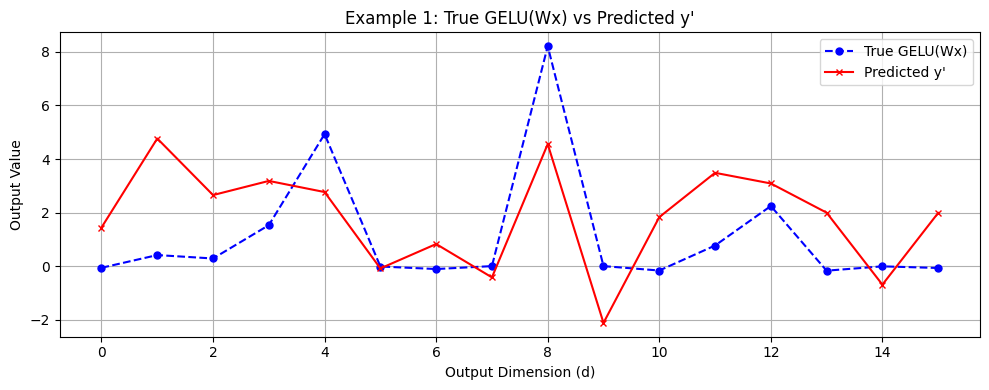
\includegraphics[width=1\linewidth]{True_and_Prediction.png}
    \label{fig:enter-label}
\end{center}

\begin{figure}
    \centering
    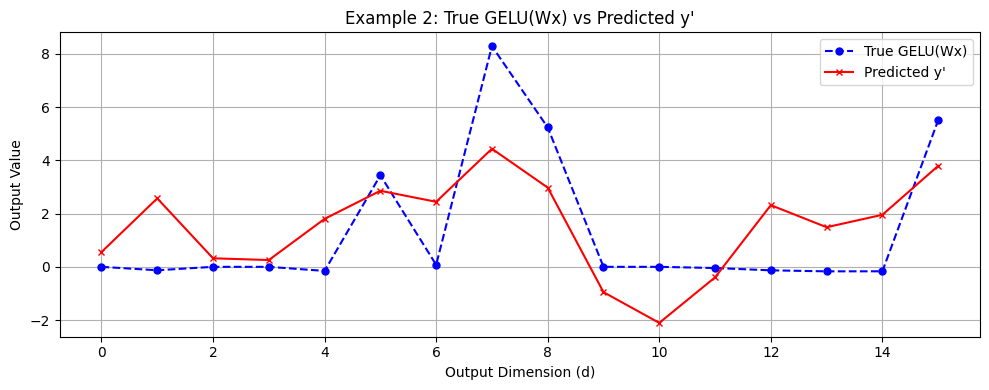
\includegraphics[width=1\linewidth]{True_and_Prediction2.png}
    \label{fig:enter-label}
\end{figure}

\begin{figure}
    \centering
    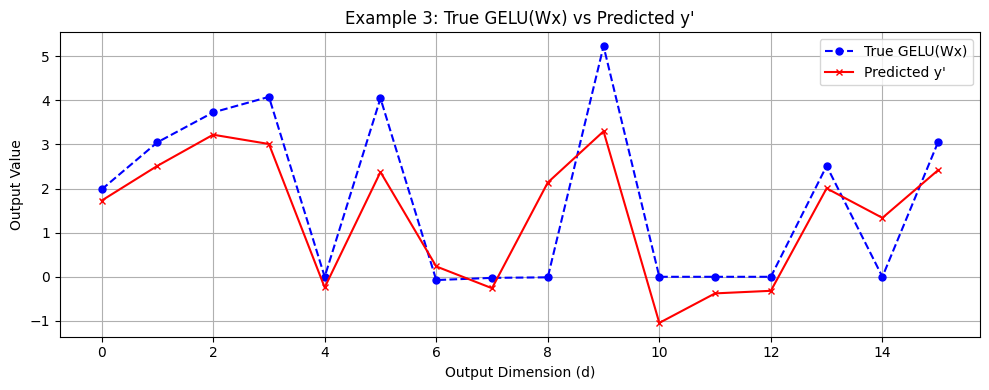
\includegraphics[width=1\linewidth]{example3.png}
    \label{fig:enter-label}
\end{figure}

\begin{figure}
    \centering
    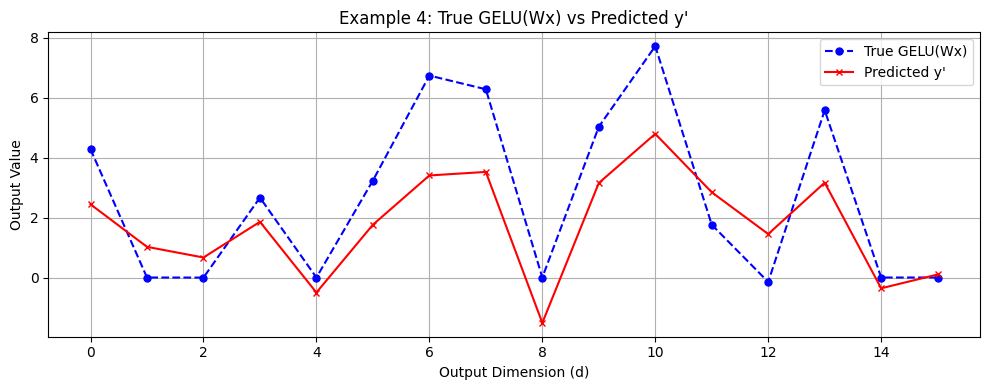
\includegraphics[width=1\linewidth]{example4.png}
    \label{fig:enter-label}
\end{figure}

\subsubsection{Training loss over steps count}
The training loss over 2000 steps is graphed, and we visualized loss curve decreases and gradually converges to the true GELU approximation with an average of $\sim$ 2.013.

\begin{figure}[h]
    \centering
    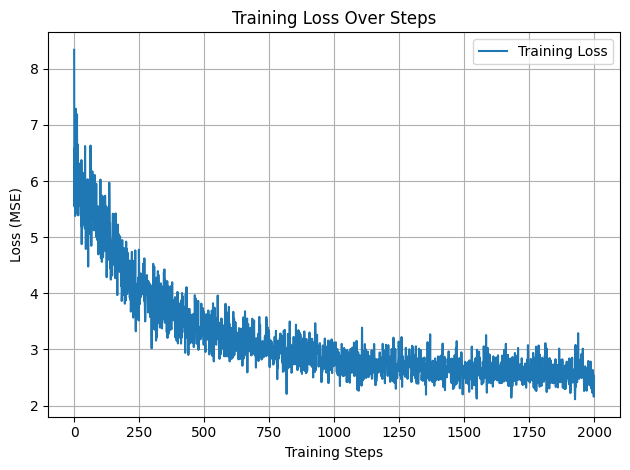
\includegraphics[width=0.7\textwidth]{training_loss.png}
    \caption{Training Loss over 2000 steps, stabilizes around 2.013}
    \label{fig:enter-label}
\end{figure}

\section{Further Exploration and Usages}
\subsection{Adoption of the two decomposed functions into transformer-based models}
As a part of further exploration, and without time constraints, our team would like to explore if decomposed functions have benefits such as accelerating model convergence time. We speculate this on the basis that current state-of-the-art transformer-based natural language processing models use GELU. 
\end{document}